\chapter{Introducción}\label{introducciuxf3n}

\section{Laboratorio de Investigación y Desarrollo de Software e Inteligencia Artificial - LIDeSIA}\label{laboratorio-de-investigaciuxf3n-y-desarrollo-de-software-e-inteligencia-artificial---lidesia}

El LIDeSIA se constituye como un espacio científico, tecnológico y sociotécnico diseñado para institucionalizar, articular y dar visibilidad a las actividades de formación, investigación y extensión en el área de las ciencias de la computación y la Inteligencia Artificial (IA).

Funciona como un dispositivo de vinculación interdisciplinaria que conecta a docentes, investigadores, estudiantes de grado y agentes externos (tanto públicos como privados) para desarrollar una estrategia integral frente a los desafíos de la revolución tecnológica. Su enfoque está fuertemente orientado hacia la adopción responsable de la IA, el uso ético, la soberanía regional y la resolución de demandas sociales y científicas.

El plan de trabajo del laboratorio se articula de manera integral a través de cuatro grandes áreas disciplinares y transversales estratégicas que abarcan desde los aspectos regulatorios hasta la infraestructura física.

La primera de estas áreas es la de Ética, Regulaciones e Impacto de la IA (ERIA), la cual se dedica a investigar las implicancias legales, sociales y éticas derivadas del uso de sistemas inteligentes. Este espacio adopta lineamientos de marcos internacionales, como los de la UNESCO y la Unión Europea, para promover buenas prácticas, identificar sesgos algorítmicos y asegurar un desarrollo tecnológico que sea responsable y seguro para la sociedad.

En el plano analítico y formal, el laboratorio cuenta con el área de Matemática para la IA (MIA). Este eje se enfoca en el estudio de los fundamentos teóricos necesarios para el aprendizaje automático, tales como el álgebra lineal, los procesos estocásticos, la optimización, la estadística y la teoría de grafos. El objetivo principal de esta línea de investigación es desarrollar modelos computacionales que no solo sean eficientes en su ejecución, sino que también cumplan con criterios de inteligibilidad y transparencia mediante la inteligencia artificial explicable.

Por el lado del soporte técnico y el procesamiento a gran escala, se despliega el área de Infraestructura Tecnológica e Ingeniería de Datos (ITID). Aquí los investigadores analizan el comportamiento de distintas arquitecturas de hardware, incluyendo unidades de procesamiento avanzado y tecnologías abiertas como RISC-V. Asimismo, se especializan en la ingeniería y gestión de macrodatos (Big Data), buscando diseñar estrategias de cómputo optimizadas que colaboren a reducir la dependencia tecnológica de la región.

Finalmente, el laboratorio impulsa el estudio de nuevas tendencias y recursos de software para IA. Esta última línea de trabajo se centra en explorar herramientas de software emergentes y en transferir los principios rigurosos de la ingeniería de sistemas hacia el ecosistema de los sistemas inteligentes. Mediante la optimización del código y la adopción de metodologías de desarrollo modernas, este eje busca garantizar la mantenibilidad, escalabilidad y eficiencia de los productos de software que integran componentes cognitivos.

\section{Ministerio Publico Fiscal de la Provincia de Córdoba - MPF}\label{ministerio-publico-fiscal-de-la-provincia-de-cuxf3rdoba---mpf}

El Ministerio Público Fiscal (MPF) de la Provincia de Córdoba es un órgano constitucional dotado de autonomía funcional y autarquía administrativa, integrado al Poder Judicial. Su función principal, bajo la dirección de la Fiscalía General, consiste en promover la actuación de la justicia en defensa de los intereses de la sociedad civil, dirigir la investigación penal preparatoria y ejercer la acción penal pública.

Para el cumplimiento operativo de la investigación de los delitos, el MPF cuenta con la Dirección General de Policía Judicial, un cuerpo técnico y científico multidisciplinar encargado de asistir a los fiscales en la recopilación, preservación y análisis de elementos de prueba.

Dentro de esta estructura auxiliar y descentralizada se ubican las Unidades Judiciales, oficinas operativas distribuidas estratégicamente que funcionan las 24 horas del día como el primer contacto entre el ciudadano y el sistema de administración de justicia penal, encargándose de la recepción de denuncias y de las actuaciones preventivas iniciales.

Este trabajo se centra específicamente en la Unidad Judicial de Accidentología Vial, que es una dependencia especializada en materia penal y vial. Su competencia se circunscribe a la intervención técnica y sumarial inmediata ante hechos que encuadren presuntamente en delitos contra la vida, la salud o la integridad física derivados de siniestros de tránsito (tales como homicidios culposos o lesiones culposas en ocasión de tránsito, tipificados en el Código Penal de la Nación). Esta unidad destaca por articular de manera directa la actuación del sumariante judicial con los gabinetes científicos especializados (accidentologos, peritos mecánicos y médicos forenses), garantizando la inmediatez y la cadena de custodia en el aseguramiento de la prueba en la escena del hecho, insumo crítico para la posterior determinación de responsabilidades penales por parte de las Fiscalías de Instrucción intervinientes.

\begin{longtable}[]{@{}
>{\centering\arraybackslash}p{(\linewidth - 2\tabcolsep) * \real{0.2984}}
  >{\centering\arraybackslash}p{(\linewidth - 2\tabcolsep) * \real{0.6642}}@{}}
\caption{Áreas del Ministerio Público Fiscal de la Provincia de Córdoba}
\label{tab:areas-del-ministerio-publico-fiscal-de-l}\\
\toprule\noalign{}
\endfirsthead
\toprule\noalign{}
\endhead
\bottomrule\noalign{}
\endlastfoot
\textbf{Nivel Operativo / Área} & \textbf{Componentes y Unidades Específicas.} \\
Alta Dirección & Fiscalía General de la Provincia y Fiscalías Generales Adjuntas. \\
Gestión Estratégica & Dirección General de Planificación y Control de Gestión; Instituto de Formación; Dirección de Infraestructura. \\
Fiscalías por Instancia & Fiscalías de Cámara y Fiscalías de Instrucción. \\
Fiscalías Especializadas & Lucha contra el Narcotráfico; Penal, Económico y Anticorrupción; Violencia Familiar; Delitos contra la Integridad Sexual; Delitos Complejos; Cibercrimen. \\
Áreas Judiciales Complementarias & Fiscalías Civiles, Comerciales, Laborales y de Familia; Fiscalías Penales Juveniles. \\
Unidades Operativas Territoriales & Unidades Judiciales (Generales); Unidades Territoriales; Unidad Fiscal de Flagrancia; Unidades Contravencionales. \\
Unidad Especializada en Siniestralidad & Unidades Judiciales de Accidentología Vial (UJ). \\
Auxiliares de la Justicia & Policía Judicial (Gabinetes de Reconstrucción Criminal y Fotografía Legal); Fuerza Policial Antinarcotráfico (FPA). \\
\end{longtable}

Fuente: Elaboración propia en base a la normativa de convenios con la FCEFyN-UNC y el portal institucional del Ministerio Público Fiscal de Córdoba

\section{LIDeSIA y MPF}\label{lidesia-y-mpf}

La relación institucional entre el Laboratorio de Investigación y Desarrollo de Software e Inteligencia Artificial (LIDeSIA) y el Ministerio Público Fiscal (MPF) de la Provincia de Córdoba se encuentra establecida en un marco jurídico formal que se denomina el Convenio de Cooperación Mutua suscrito en el año 2017. Este vínculo estratégico se profundizó a través del Anexo I, ratificado mediante la Resolución Decanal 480/2017, el cual establece un Convenio Específico de Colaboración Recíproca orientado a la investigación, desarrollo y transferencia de tecnología en el campo de la inteligencia artificial aplicada al ámbito jurídico y forense. El objeto de este acuerdo permite la creación de herramientas de software destinadas a mejorar la gobernanza de datos y facilitar la toma de decisiones dentro de la estructura del MPF.

En cuanto a la trayectoria de colaboración, LIDeSIA ha desarrollado con anterioridad diversas soluciones técnicas que sirven de base para las investigaciones actuales. El desarrollo inicial del Sistema de Gestión de Siniestros Viales (SGAV) fue llevado a cabo por equipos pertenecientes al laboratorio, integrados específicamente por estudiantes de intercambio provenientes de Francia y México bajo la coordinación de una directora de proyectos de LIDeSIA, este trabajo consistió en la creación de una plataforma web diseñada para la visualización, caracterización y análisis descriptivo de datos reales sobre accidentología vial en la ciudad de Córdoba. La arquitectura técnica fue alojada en el Centro de Cómputo de Alto Desempeño (CCAD) de la Universidad Nacional de Córdoba y se estructuró siguiendo los lineamientos de la norma ISO 42001 para la gestión de sistemas de inteligencia artificial. Esta colaboración preexistente al momento de comenzar este proyecto fue especialmente relevante dado que permitió la recopilación de un set de datos reales desde comienzos del año 2022, los cuales fueron fundamentales para que en octubre de 2023 se iniciara el proyecto titulado ``Inteligencia Artificial para atender a la problemática de siniestros viales'' bajo la convocatoria PPIDTA-IA de la SECYT. Este proyecto en particular fue motivo de las prácticas profesionales supervisadas de los autores, el desarrollo que se realizó en su momento fue crítico para consolidar el producto y dejar bases sólidas a partir de las cuales se continuarán añadiendo nuevas funcionalidades y características.

La continuidad de este trabajo conjunto ha permitido evolucionar desde aplicaciones de gestión de datos hacia sistemas de alerta temprana y modelos predictivos de siniestralidad, consolidando una sinergia orientada a la transformación digital y la implementación de inteligencia artificial en la administración de justicia.

\section{Surgimiento del proyecto}\label{surgimiento-del-proyecto}

La idea de este proyecto surge durante el desarrollo de las prácticas profesionales supervisadas antes mencionadas, donde se trabajó desde LIDeSIA con un sistema de gestión de siniestralidad vial que cuenta con funcionalidades para el análisis de datos, la visualización y caracterización de los siniestros. Durante la etapa de pruebas de usuario, y producto de la interacción con usuarios finales, se evidenció la necesidad de incorporar funcionalidades con capacidades predictivas.

El Ministerio Público Fiscal tiene distintos recursos para asignar según las funciones y responsabilidades de cada área, en el caso de la unidad de accidentología vial existen algunas particularidades dada la naturaleza de la misma, por ejemplo la interacción con los oficiales de justicia, peritos, policía de la provincia de Córdoba, funcionarios municipales, personal de clínicas y hospitales que prestan servicios a la población de la ciudad de Córdoba. Estos y otros recursos deben ser planificados, coordinados y controlados para que estén disponibles 24 horas todos los días del año, es en este contexto de gran complejidad donde toma especial valor tener algún tipo de capacidad predictiva que permita proveer a los usuarios un grado de soporte a la toma de decisiones en situaciones de incertidumbre, bien sea porque permite anticiparse o facilitar la decisión.

A modo introductorio se mencionará que los accidentes son clasificados por su gravedad (leves, graves, graves y gravísimas) siendo el motivo de esta clasificación el proceso penal que enfrentará el potencial responsable del accidente. Dependiendo de este tipo de lesiones el proceso puede variar, por ejemplo, se sabe que un gran porcentaje de los accidentes que tienen lesiones graves y gravísimas terminan con la muerte de la víctima al cabo de un determinado tiempo, esto requiere que el personal sea más exhaustivo, peritos o especialistas específicos para el tipo de accidente y un proceso diferente a nivel penal que si hubiese sido una lesión leve. En este sentido sería de especial utilidad que el personal del MPF pudiera tener un sistema que alerte o estime de manera anticipada el riesgo de que ocurran accidentes para distintos momentos del día, esto les permitirá gestionar mejor los recursos que tienen disponibles para prestar su servicio.

\section{Procedimiento judicial ante un siniestro}\label{procedimiento-judicial-ante-un-siniestro}

% TODO(caption): esta figura no tenía leyenda en el original, completar.
\begin{figure}[htbp]
\centering
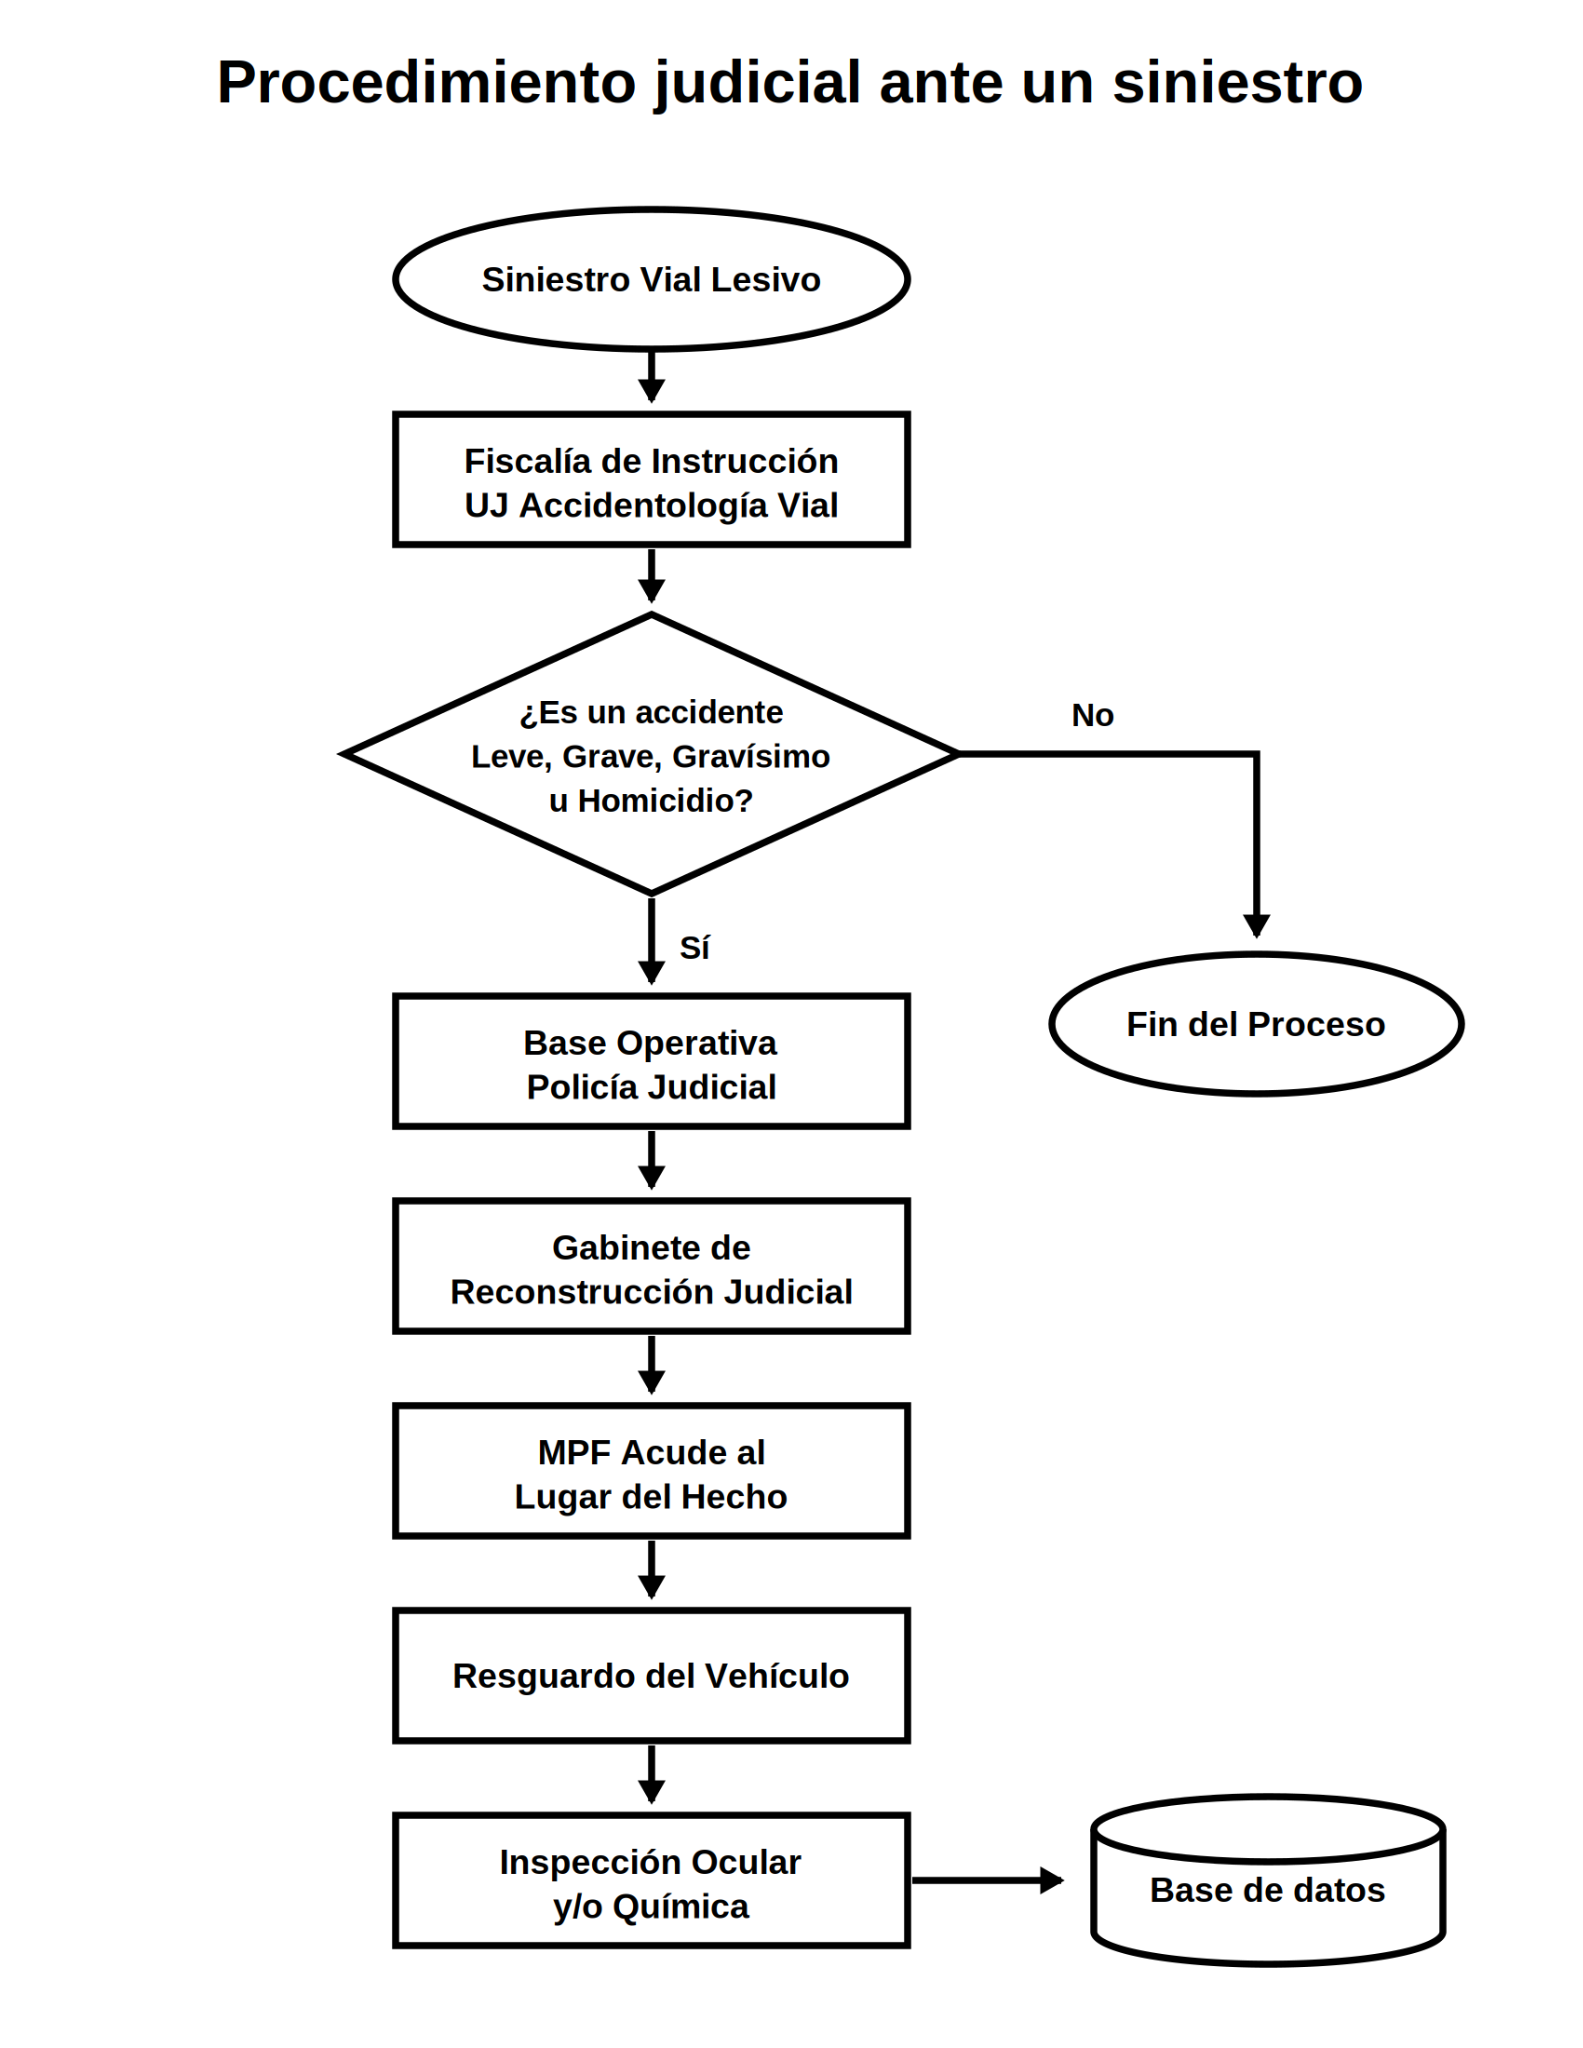
\includegraphics[width=\linewidth]{imagenes/image13.png}
\caption{Descripción pendiente}
\label{fig:procedimiento-judicial-siniestro}
\end{figure}

El procedimiento judicial tanto en su dimensión administrativa como pericial ante un siniestro vial se inicia con la toma de conocimiento por parte de la fiscalía de instrucción, que opera específicamente a través de las unidades judiciales, en este caso en particular actúa la unidad judicial de accidentología vial (UJ), las cuales practican los primeros actos de la investigación penal preparatoria. Según la calificación legal del hecho, que puede comprender desde lesiones leves hasta homicidio, puede solicitarse la intervención de la base operativa de Policía Judicial para desplegar los recursos técnicos de los gabinetes de reconstrucción criminal y fotografía legal de manera inmediata en el lugar del suceso. Tras realizar los trabajos y los procesos específicos para la preservación de la escena, el vehículo es resguardado en una Unidad Judicial, acto seguido la oficina técnica realiza las inspecciones oculares y químicas correspondientes.

En paralelo, se desarrolla un proceso de gestión documental y carga de información donde personal administrativo, estudiantes de derecho o abogados completan un formulario inicial e integran la declaración del agente policial interviniente. Esta etapa es crítica dentro del proceso dado que es el momento en cual comienzan a adquirirse los datos y la recopilación de estos registros que constituye la formación del conjunto de datos o dataset. En última instancia, esta sistematización digital permite que la información recolectada funcione como el insumo base para el entrenamiento de modelos de inteligencia artificial, en este sentido hay que destacar otro aspecto de vital importancia y es el referido a el tiempo que pasa entre el accidente y la carga de datos en el dataset. Cuando se trabaja con sistemas que realizan forecasting la disponibilidad de información en función del tiempo es crítica, en especial en problemas donde necesitamos agregar los datos en bloques discretos de tiempo. Este aspecto se desarrolla con suficiente profundidad más adelante, en cuanto a su influencia en el proceso se contempla esta restricción tanto para la decisión del modelo, la estructura de los dataset, la arquitectura del sistema en su conjunto y los requerimientos y funcionalidades del producto.

\section{Objetivo del proyecto}\label{objetivo-del-proyecto}

Este proyecto integrador consiste en el diseño de un producto end to end, comenzando desde la transformación de los datos, el desarrollo de modelos impulsados por inteligencia artificial y la implementación de los mismos a nivel MVP en un sistema integrado y desplegado que pueda ser consumido por el usuario final.

Este producto será concebido desde una mirada transversal y con particular interés en los aspectos que competen al campo de la ingeniería industrial, en ese sentido se puede destacar el uso de metodologías ágiles para la gestión del proyecto de desarrollo, las competencias relacionadas al trabajo con equipos de múltiples disciplinas en especial las que no están vinculadas a las ciencias exactas, el enfoque sistémico para mejorar un proceso donde están implicados no sólo aspectos tecnológicos sino también humanos y normativos. Otro campo de la ingeniería industrial que se tendrá en cuenta para los objetivos de este producto es el relacionado a los sistemas de gestión, en particular para este caso es la Norma ISO/IEC 42001 para el desarrollo responsable, transparente y ético.

De manera general y sin perjuicio de lo antes mencionado, este trabajo incluirá un análisis de los principales aspectos de la gestión de un producto impulsado por inteligencia artificial para forecasting de accidentes viales, como gestión de riesgos, análisis y definición de requisitos, escalabilidad del producto, evaluación de impacto y la documentación asociada a sus partes.
